%% Beginning of file 'sample631.tex'
%%
%% Modified 2022 May  
%%
%% This is a sample manuscript marked up using the
%% AASTeX v6.31 LaTeX 2e macros.
%%
%% AASTeX is now based on Alexey Vikhlinin's emulateapj.cls 
%% (Copyright 2000-2015).  See the classfile for details.

%% AASTeX requires revtex4-1.cls and other external packages such as
%% latexsym, graphicx, amssymb, longtable, and epsf.  Note that as of 
%% Oct 2020, APS now uses revtex4.2e for its journals but remember that 
%% AASTeX v6+ still uses v4.1. All of these external packages should 
%% already be present in the modern TeX distributions but not always.
%% For example, revtex4.1 seems to be missing in the linux version of
%% TexLive 2020. One should be able to get all packages from www.ctan.org.
%% In particular, revtex v4.1 can be found at 
%% https://www.ctan.org/pkg/revtex4-1.

%% The first piece of markup in an AASTeX v6.x document is the \documentclass
%% command. LaTeX will ignore any data that comes before this command. The 
%% documentclass can take an optional argument to modify the output style.
%% The command below calls the preprint style which will produce a tightly 
%% typeset, one-column, single-spaced document.  It is the default and thus
%% does not need to be explicitly stated.
%%
%% using aastex version 6.3
%\documentclass[linenumbers]{aastex631}
\documentclass[preprint2]{aastex631}


%% The default is a single spaced, 10 point font, single spaced article.
%% There are 5 other style options available via an optional argument. They
%% can be invoked like this:
%%
%% \documentclass[arguments]{aastex631}
%% 
%% where the layout options are:
%%
%%  twocolumn   : two text columns, 10 point font, single spaced article.
%%                This is the most compact and represent the final published
%%                derived PDF copy of the accepted manuscript from the publisher
%%  manuscript  : one text column, 12 point font, double spaced article.
%%  preprint    : one text column, 12 point font, single spaced article.  
%%  preprint2   : two text columns, 12 point font, single spaced article.
%%  modern      : a stylish, single text column, 12 point font, article with
%% 		  wider left and right margins. This uses the Daniel
%% 		  Foreman-Mackey and David Hogg design.
%%  RNAAS       : Supresses an abstract. Originally for RNAAS manuscripts 
%%                but now that abstracts are required this is obsolete for
%%                AAS Journals. Authors might need it for other reasons. DO NOT
%%                use \begin{abstract} and \end{abstract} with this style.
%%
%% Note that you can submit to the AAS Journals in any of these 6 styles.
%%
%% There are other optional arguments one can invoke to allow other stylistic
%% actions. The available options are:
%%
%%   astrosymb    : Loads Astrosymb font and define \astrocommands. 
%%   tighten      : Makes baselineskip slightly smaller, only works with 
%%                  the twocolumn substyle.
%%   times        : uses times font instead of the default
%%   linenumbers  : turn on lineno package.
%%   trackchanges : required to see the revision mark up and print its output
%%   longauthor   : Do not use the more compressed footnote style (default) for 
%%                  the author/collaboration/affiliations. Instead print all
%%                  affiliation information after each name. Creates a much 
%%                  longer author list but may be desirable for short 
%%                  author papers.
%% twocolappendix : make 2 column appendix.
%%   anonymous    : Do not show the authors, affiliations and acknowledgments 
%%                  for dual anonymous review.
%%
%% these can be used in any combination, e.g.
%%
%% \documentclass[twocolumn,linenumbers,trackchanges]{aastex631}
%%
%% AASTeX v6.* now includes \hyperref support. While we have built in specific
%% defaults into the classfile you can manually override them with the
%% \hypersetup command. For example,
%%
%% \hypersetup{linkcolor=red,citecolor=green,filecolor=cyan,urlcolor=magenta}
%%
%% will change the color of the internal links to red, the links to the
%% bibliography to green, the file links to cyan, and the external links to
%% magenta. Additional information on \hyperref options can be found here:
%% https://www.tug.org/applications/hyperref/manual.html#x1-40003
%%
%% Note that in v6.3 "bookmarks" has been changed to "true" in hyperref
%% to improve the accessibility of the compiled pdf file.
%%
%% If you want to create your own macros, you can do so
%% using \newcommand. Your macros should appear before
%% the \begin{document} command.
%%
\newcommand{\vdag}{(v)^\dagger}
\newcommand\aastex{AAS\TeX}
\newcommand\latex{La\TeX}

%% Reintroduced the \received and \accepted commands from AASTeX v5.2
%\received{March 1, 2021}
%\revised{April 1, 2021}
%\accepted{\today}

%% Command to document which AAS Journal the manuscript was submitted to.
%% Adds "Submitted to " the argument.
%\submitjournal{PSJ}

%% For manuscript that include authors in collaborations, AASTeX v6.31
%% builds on the \collaboration command to allow greater freedom to 
%% keep the traditional author+affiliation information but only show
%% subsets. The \collaboration command now must appear AFTER the group
%% of authors in the collaboration and it takes TWO arguments. The last
%% is still the collaboration identifier. The text given in this
%% argument is what will be shown in the manuscript. The first argument
%% is the number of author above the \collaboration command to show with
%% the collaboration text. If there are authors that are not part of any
%% collaboration the \nocollaboration command is used. This command takes
%% one argument which is also the number of authors above to show. A
%% dashed line is shown to indicate no collaboration. This example manuscript
%% shows how these commands work to display specific set of authors 
%% on the front page.
%%
%% For manuscript without any need to use \collaboration the 
%% \AuthorCollaborationLimit command from v6.2 can still be used to 
%% show a subset of authors.
%
%\AuthorCollaborationLimit=2
%
%% will only show Schwarz & Muench on the front page of the manuscript
%% (assuming the \collaboration and \nocollaboration commands are
%% commented out).
%%
%% Note that all of the author will be shown in the published article.
%% This feature is meant to be used prior to acceptance to make the
%% front end of a long author article more manageable. Please do not use
%% this functionality for manuscripts with less than 20 authors. Conversely,
%% please do use this when the number of authors exceeds 40.
%%
%% Use \allauthors at the manuscript end to show the full author list.
%% This command should only be used with \AuthorCollaborationLimit is used.

%% The following command can be used to set the latex table counters.  It
%% is needed in this document because it uses a mix of latex tabular and
%% AASTeX deluxetables.  In general it should not be needed.
%\setcounter{table}{1}

%%%%%%%%%%%%%%%%%%%%%%%%%%%%%%%%%%%%%%%%%%%%%%%%%%%%%%%%%%%%%%%%%%%%%%%%%%%%%%%%
%%
%% The following section outlines numerous optional output that
%% can be displayed in the front matter or as running meta-data.
%%
%% If you wish, you may supply running head information, although
%% this information may be modified by the editorial offices.
%\shorttitle{AASTeX v6.3.1 Sample article}
%\shortauthors{Schwarz et al.}
%%
%% You can add a light gray and diagonal water-mark to the first page 
%% with this command:
%% \watermark{text}
%% where "text", e.g. DRAFT, is the text to appear.  If the text is 
%% long you can control the water-mark size with:
%% \setwatermarkfontsize{dimension}
%% where dimension is any recognized LaTeX dimension, e.g. pt, in, etc.
%%
%%%%%%%%%%%%%%%%%%%%%%%%%%%%%%%%%%%%%%%%%%%%%%%%%%%%%%%%%%%%%%%%%%%%%%%%%%%%%%%%
%\graphicspath{{./}{figures/}}
\graphicspath{ {../figures/} }
%% This is the end of the preamble.  Indicate the beginning of the
%% manuscript itself with \begin{document}.

\begin{document}

\title{Gaia Parallax Distances: What Can Go Wrong and How to Fix It}


%% LaTeX will automatically break titles if they run longer than
%% one line. However, you may use \\ to force a line break if
%% you desire. In v6.31 you can include a footnote in the title.

%% A significant change from earlier AASTEX versions is in the structure for 
%% calling author and affiliations. The change was necessary to implement 
%% auto-indexing of affiliations which prior was a manual process that could 
%% easily be tedious in large author manuscripts.
%%
%% The \author command is the same as before except it now takes an optional
%% argument which is the 16 digit ORCID. The syntax is:
%% \author[xxxx-xxxx-xxxx-xxxx]{Author Name}
%%
%% This will hyperlink the author name to the author's ORCID page. Note that
%% during compilation, LaTeX will do some limited checking of the format of
%% the ID to make sure it is valid. If the "orcid-ID.png" image file is 
%% present or in the LaTeX pathway, the OrcID icon will appear next to
%% the authors name.
%%
%% Use \affiliation for affiliation information. The old \affil is now aliased
%% to \affiliation. AASTeX v6.31 will automatically index these in the header.
%% When a duplicate is found its index will be the same as its previous entry.
%%
%% Note that \altaffilmark and \altaffiltext have been removed and thus 
%% can not be used to document secondary affiliations. If they are used latex
%% will issue a specific error message and quit. Please use multiple 
%% \affiliation calls for to document more than one affiliation.
%%
%% The new \altaffiliation can be used to indicate some secondary information
%% such as fellowships. This command produces a non-numeric footnote that is
%% set away from the numeric \affiliation footnotes.  NOTE that if an
%% \altaffiliation command is used it must come BEFORE the \affiliation call,
%% right after the \author command, in order to place the footnotes in
%% the proper location.
%%
%% Use \email to set provide email addresses. Each \email will appear on its
%% own line so you can put multiple email address in one \email call. A new
%% \correspondingauthor command is available in V6.31 to identify the
%% corresponding author of the manuscript. It is the author's responsibility
%% to make sure this name is also in the author list.
%%
%% While authors can be grouped inside the same \author and \affiliation
%% commands it is better to have a single author for each. This allows for
%% one to exploit all the new benefits and should make book-keeping easier.
%%
%% If done correctly the peer review system will be able to
%% automatically put the author and affiliation information from the manuscript
%% and save the corresponding author the trouble of entering it by hand.

%\correspondingauthor{August Muench}
%\email{greg.schwarz@aas.org, gus.muench@aas.org}


\author{Michael Tauraso}



%% Note that the \and command from previous versions of AASTeX is now
%% depreciated in this version as it is no longer necessary. AASTeX 
%% automatically takes care of all commas and "and"s between authors names.

%% AASTeX 6.31 has the new \collaboration and \nocollaboration commands to
%% provide the collaboration status of a group of authors. These commands 
%% can be used either before or after the list of corresponding authors. The
%% argument for \collaboration is the collaboration identifier. Authors are
%% encouraged to surround collaboration identifiers with ()s. The 
%% \nocollaboration command takes no argument and exists to indicate that
%% the nearby authors are not part of surrounding collaborations.

%% Mark off the abstract in the ``abstract'' environment. 
\begin{abstract}
With the unique and revolutionary measurements of the Gaia era affecting many areas of the study of the structure and history of the Milky Way, this paper looks at the parallax distances and explores the high level causes of spurious parallaxes in Gaia DR3, as well as exploring some approaches for using these parallaxes and the astrometric solution as a whole to measure distance.
\end{abstract}

%% Keywords should appear after the \end{abstract} command. 
%% The AAS Journals now uses Unified Astronomy Thesaurus concepts:
%% https://astrothesaurus.org
%% You will be asked to selected these concepts during the submission process
%% but this old "keyword" functionality is maintained in case authors want
%% to include these concepts in their preprints.
%\keywords{Classical Novae (251) --- Ultraviolet astronomy(1736) --- History of astronomy(1868) --- Interdisciplinary astronomy(804)}

%% From the front matter, we move on to the body of the paper.
%% Sections are demarcated by \section and \subsection, respectively.
%% Observe the use of the LaTeX \label
%% command after the \subsection to give a symbolic KEY to the
%% subsection for cross-referencing in a \ref command.
%% You can use LaTeX's \ref and \label commands to keep track of
%% cross-references to sections, equations, tables, and figures.
%% That way, if you change the order of any elements, LaTeX will
%% automatically renumber them.
%%
%% We recommend that authors also use the natbib \citep
%% and \citet commands to identify citations.  The citations are
%% tied to the reference list via symbolic KEYs. The KEY corresponds
%% to the KEY in the \bibitem in the reference list below. 

\section{Introduction} \label{sec:intro}

% TODO':
% Proofreading pass
% Fill in numbers in introduction (or rephrase to remove them)
% Make sure all terms are introduced, especially gaia EDR3 and its cozy relationship with DR3 that results in so many comparisons being done against EDR3 astrometrics when we really mean DR3

ESA's Gaia mission has been a boon to the study of the Milky Way. At time of writing Data Release 3 (DR3) has a publically searchable catalog of some $~1.8$ billion sources with $88\%$ of those having a high quality astrometric solution, and some $81\%$ containing a published astrometric parallax. In comparison with Gaia's predecessor sattellite, Hipparcos, this is over a $10^4$ fold increase in the number of sources, and over a $100$ fold increase in parallax precision \cite{perrymanHistory2012}

The detailed study of the structure of the milky way benefits greatly from the enhanced precision of these parallax measures; however Gaia's astrometric parallaxes contain an estimated $3.04$ million parallaxes that are negative and known to high precision\footnote{\texttt{parallax\_over\_error < -5}}. These spurious astrometric solutions are more numerous than would be expected from the instrumentation precision of the spacecraft \cite{fabriciusGaia2021}. The interpretation of these parallax values as distances is the subject of some study. Their presence in the published Gaia data is in some ways a commitment to a certain predictability in the structure of astrometric data processing. This discipline has independent scientific value outside of the accuracy of the data released in DR3.

In this paper, section \ref{sec:parallax} will sketch the process by which Gaia parallaxes are determined, and section \ref{sec:wrong} will discuss some of the ways this process can lead to a erronious (or even negative) parallax. Section \ref{sec:distance} will sketch and compare efforts to derive distances from DR3 parallaxes. Section \ref{sec:improvement} will discuss improvements expected in Gaia's upcoming data release (DR4), as well as comparing DR3 with the prior major data release (DR2). Finally, Section \ref{sec:unorthodox} will conclude by summarizing an unorthodox use of the astrometric solution which is enabled by Gaia's data processing discipline.

\section{How Gaia Measures Parallax} \label{sec:parallax}

The standard introductory treatment of parallax considers the apex angle of a giant triangle subtended by two ends of the earth's orbit and a distant star. While pedagogically interesting and trigonometrically correct, this view pales in comparison to the complexity measuring parallaxes for nearly 2 billion sources detectable from a modern space telescope. The Gaia spacecraft sits in a Lissajous orbit at the Earth-Sun L2 Lagrange point. Gaia's two telescopes, separated by a basic angle shown in figure \ref{fig:scanninglaw}, scan the sky as the satellite rotates. As the telescope rotates, sources of light across the universe shine on to CCD detectors for each telescope as shown by the yellow star in figure \ref{fig:ccd}. The times of these transits and the response of the CCDs are recorded.

\begin{figure}
	\includegraphics[width=0.49\columnwidth]{scanninglaw.png} \includegraphics[width=0.49\columnwidth]{gaiaccd.png}
	\caption{Gaia Scan illustration (left) and Gaia CCD schematic (right) \citep{collaborationGaia2016}}
	 \label{fig:scanninglaw} \label{fig:ccd}
\end{figure}

The first steps of this analysis are focused on constructing a frame of reference for the astronomic observations and accurately placing the spacecraft and its instruments within that reference frame. Well known astronomic sources with predictable behavior are identified algorithmically and used as points of reference to calibrate detailed mathematial models of the spacecraft's location over time. Once this model of the spacecraft is calibrated, it is used to convert timed transit events to sky locations and times where a source was observed. The time that a source passes by each telescope is critical, because the time that each source appears and leaves the field of view of the spacecraft is an additional piece of information that allows its sky location to be inferred with greater accuracy

\begin{figure}
	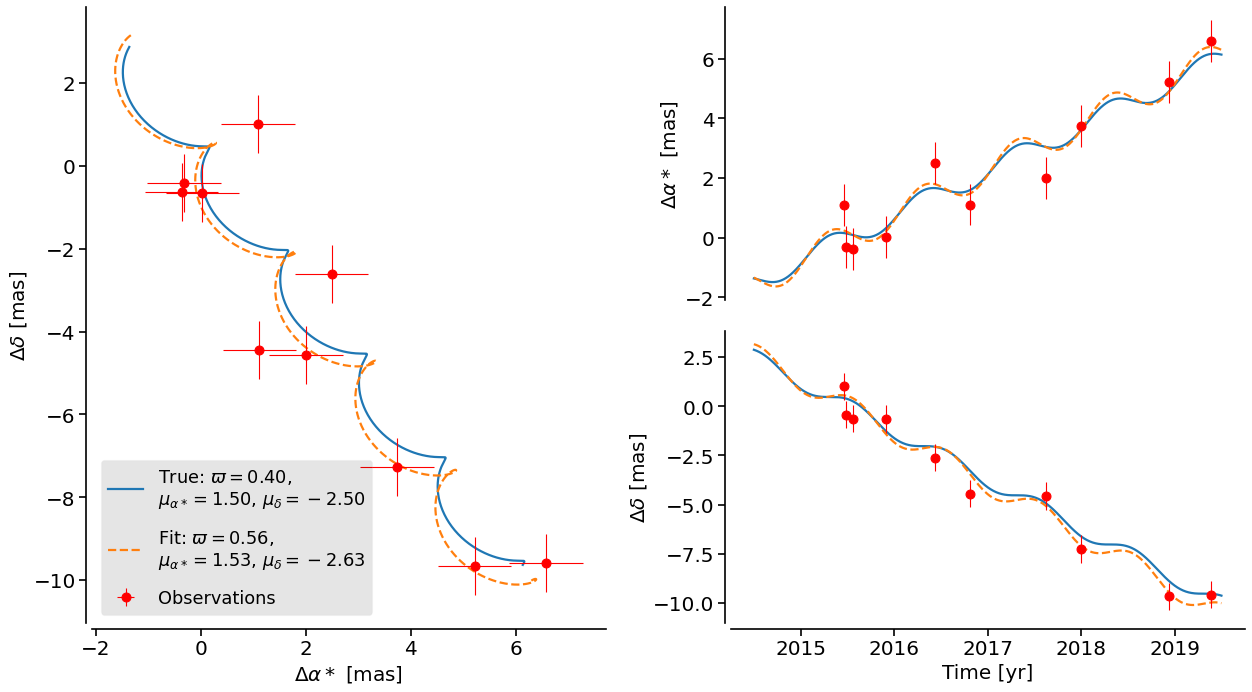
\includegraphics[width=\columnwidth]{astrometric-good.png}
	\caption{A simplified but representative astrometric curve fit. Simulated star location is in blue, simulated measurements are in red, and the fit curve is orange. The error bars are of representative size to Gaia's data. Actual and fit parameters for proper motion and Parallax are reported on the plot. Simulation was generated by author with code from \cite{luriGaia2018}}
	\label{fig:goodfit}
\end{figure}

These observations must then be grouped algorithmically, such that each group of observations is identified as being from the same source in the night sky. Parallaxes then flow from a least-squares fit of a linear model to each group of observations identified with a particular source. A simplified and simulated view of such a curve fit is shown in Figure \ref{fig:goodfit}. 

Each gaia source includes around 200 observations, and the published astrometric parameters, errors and correlations flow directly from this curve fit. The ideal case for this pipeline is a high quality 5-parameter fit, so called because the 5 astrometric parameters Right Ascension ($\alpha$), Declination ($\delta$), Right Ascension Proper Motion ($\mu_\alpha$), Declination Proper Motion ($\mu_\delta$), and Parallax ($\bar{\omega}$) are determined\footnote{Radial Velocity ($v_r$) is unmentioned here, because radial velocity is determined spectroscopically, and is used as input data to the curve fit in DR3 where it is available. While in theory $v_r$ could be an output of an astrometric curve fit, in practice this method yields useful results only for the closest and brightest sources\citep{lindegrenGaia2021a}.} by the least squares fit\citep{lindegrenGaia2021a}.

There can be issues with the veracity of this fit. Gaia's CCD instrument and telescope have non-linear response to different frequences of light, and it is well known that objects in the sky are not monochromatic. These two effects together affect the calibration of the instrument, because there are chromatic effects that affect where, when, and how much a given source is recorded on the CCD. Gaia corrects for these effects using a model that takes as input a single color, reported in the published data as \texttt{nu\_eff\_used\_in\_astrometry}. In the case where this color can be determined from spectral observations, and the resulting 5 parameter fit is of sufficiently high quality, the 5-parameter fit is reported.

In the case that the 5-parameter fit is not high enough quality to be reported, Gaia Astrometry falls back to either a 6 parameter fit or a 2 parameter fit. The 6 parameter fit treats \texttt{nu\_eff\_used\_in\_astrometry} as an additional unknown taking part of the least squares fit. The value found by the curve fit is reported in the database as \texttt{pseudocolor}. Typically very bright and very dim sources require this treatement for different reasons. Dim sources because there is not enough light to determine their true color. Bright sources end up having a 6-parameter fit because their 5-parameter fit is uncertain as their light is washing out much of the positional precision that Gaia would otherwise have\footnote{Researchers familiar with the DR2 data may note it contains several close, high proper motion, bright sources. These reportedly arose from falling back to a 6-parameter fit for a bright source with high error in its 5-parameter fit. The acceptance parameters for the 5-parameter sources were incorrectly tuned for bright sources in DR2; however, this error has been corrected in DR3 with a $G$ magnitude dependent criteria \citep{lindegrenGaia2021a}.}. 2-parameter fits (only $\alpha$ and $\delta$) are reported when neither 5-parameter nor 6-parameter fits reach the desired level of quality.

\section{What can go wrong?} \label{sec:wrong}

The process of source identification is possibly the most error-prone step in the entire astrometric pipeline, involving both components on-spacecraft that initially identify sources and a large amount of earthbound data analysis. Dim sources in crowded fields are particularly suceptible to source misidentification; however, there is a long list of astrophysical phenomena, mostly affecting dim objects, which can cause a source misidentification error. Tracking down and improving the source identification algorithm is an area of nontrivial current work.% Cite the source identification paper?
% TODO, you bitched out on characterizing this in the preso beyond a laundry list You might need to expand here, or you could just write in a laundry list

% Assuming the part above is written:
In addition to source identification issues, there are astrophysical phenomena that can cause a correctly identified source to not fit the linear 5 parameter model. Some of these have a somewhat mean-reverting property to linear motion such as binary systems, gravitationally lensed sources, and sources with dark companions. Others, such as stellar close encounters, and exceptionally fast sources have motion that simply diverges from the underlying model. These types of systems can cause a low quality or even a spurious curve fit depending on the magnitude of the effect and the timing of observations. The distribution of these different sorts of fits, as well as the fraction of them that are spurious are illustrated in Figure \ref{fig:spuriousfraction}. 
\begin{figure}
	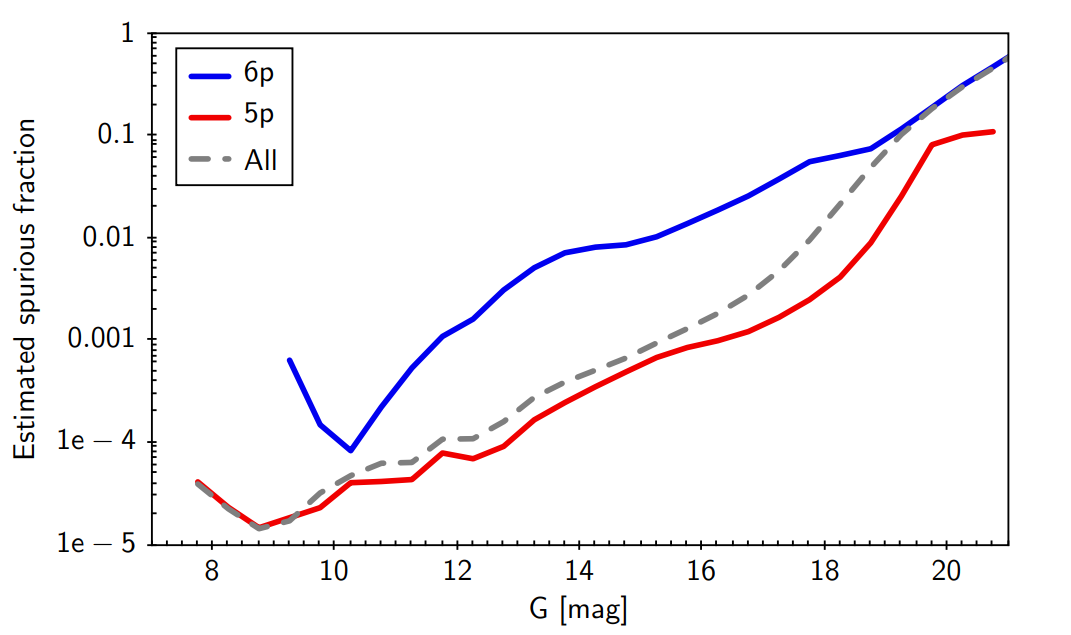
\includegraphics[width=0.56\columnwidth]{spuriousfraction.png}
	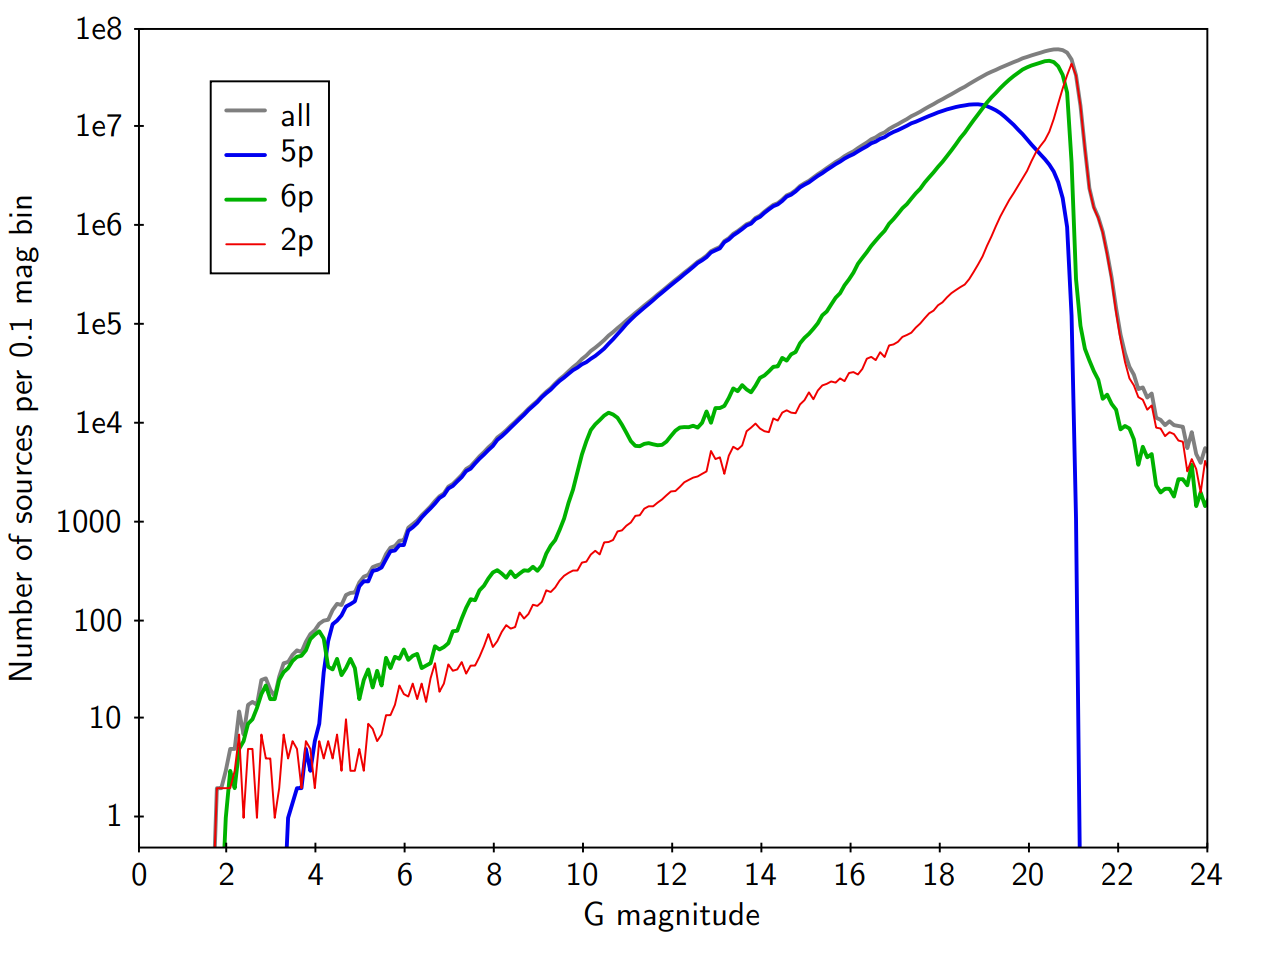
\includegraphics[width=0.42\columnwidth]{magdistEDR3.png}

	\caption{Left: Estimated fraction of spurious astrometric solutions by type in EDR3 \citep{fabriciusGaia2021}. Right: Total number of astrometric solutions by type in EDR3 by $G$ magnitude \citep{lindegrenGaia2021a}.}
	\label{fig:spuriousfraction}
\end{figure}

Even if source identification works and the source moves linearly over the observation timescale, you can still have a curve fit that is simply wrong due to the timing and uncertainty in the observations. Many negative parallaxes fall into this category. Figure \ref{fig:badfit} shows a bad fit for a simulated star, yielding a negative parallax. In this figure, the ``measured'' data points were derived from a simulation of a star with linear motion, and normally distributed measurement uncertainties.

\begin{figure}
	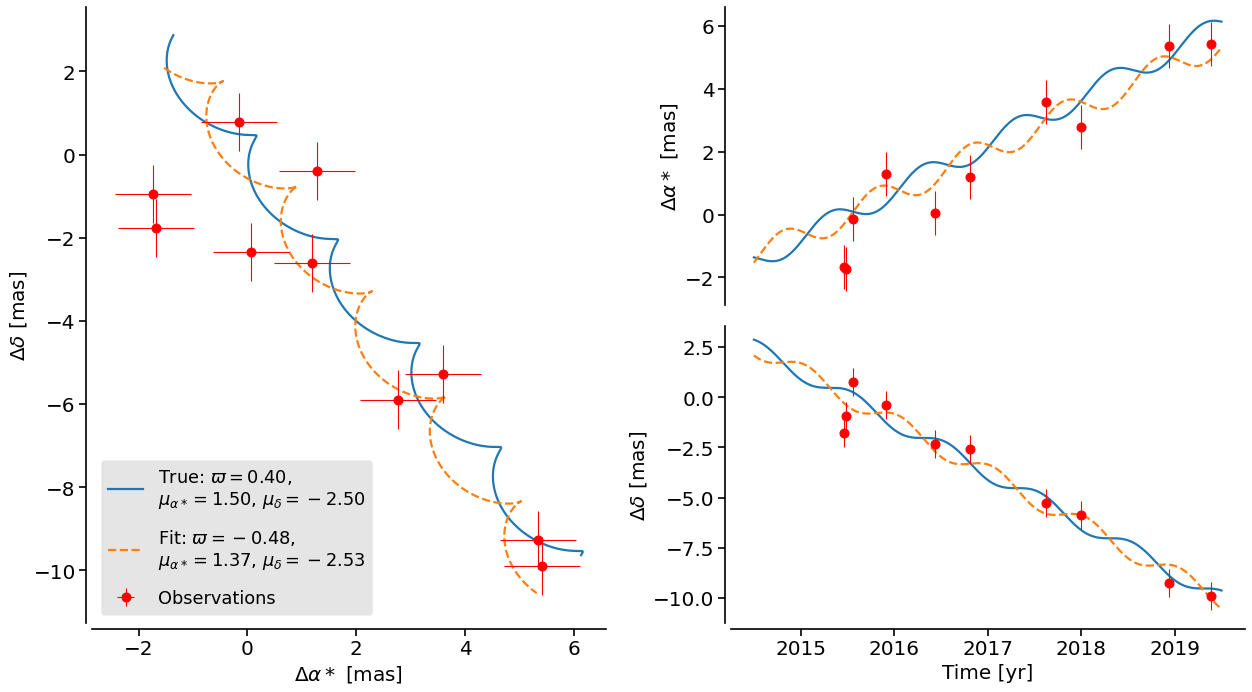
\includegraphics[width=\columnwidth]{astrometric-bad.png}
	\caption{Same as figure \ref{fig:goodfit}, except the fit is to a negative parallax value. Note the orange curve (fit) differs from the blue (actual) by a phase of $\pi$. Figure generated from code in \cite{luriGaia2018}}
	\label{fig:badfit}
\end{figure}


% Rename this section header or remove
%\section{What data is in DR3?} \label{sec:data}

Spurious astrometric solutions can vary greatly in terms of quality. While every negative parallax is definitely spurious, there are also spurious astrometric solutions that generate slightly-wrong values, many of which are within the formal errors for the reported astrometric parameters. There is ultimately still information about distance in some of these spurious solutions. For example, one step in verifying the calibration of the astrometric pipeline is computing the parallaxes for several known quasar sources\citep{luriGaia2018}. These parallaxes ought all be zero, but they are in-fact normally distributed around zero and half of them are negative! Determining whether an astrometric parallax has information is primarily an issue of looking at both the parallax value and the error estimate. When the error is small relative to the value, there is a much greater chance that even a negative parallax has information.

\begin{figure}
	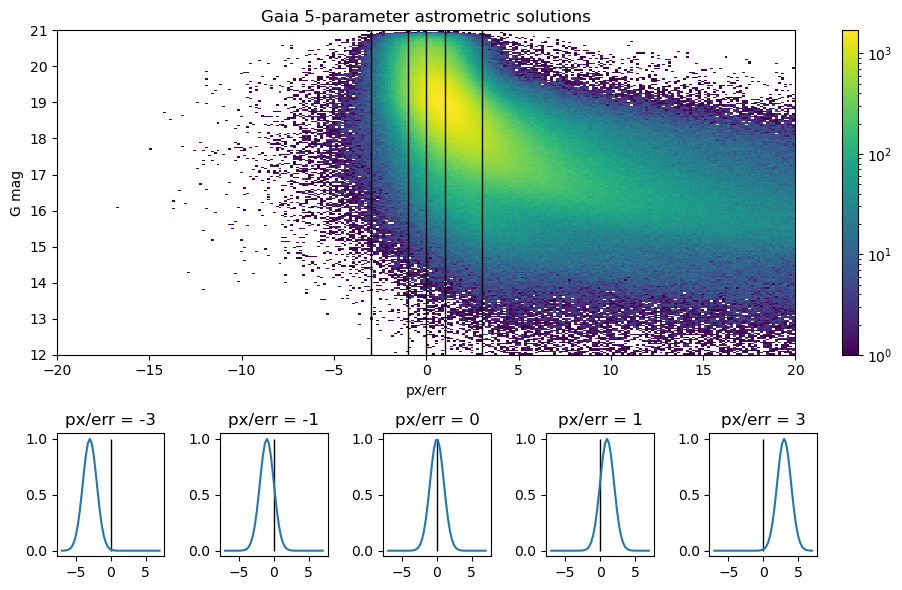
\includegraphics[width=\columnwidth]{poe_map.png}
	\caption{Histogram of Gaia DR3 5-parameter solutions by \texttt{parallax\_over\_error} measure and $G$ magnitude. Lower plots show example normal distributions for parallax measurements implied by selected \texttt{parallax\_over\_error} values. These same selected values are marked on the main plot by the black vertical lines. Data from \cite{collaborationGaia2022}}
	\label{fig:dr3poe}
\end{figure}

Figure \label{fig:dr3poe} shows a histogram of a randomly selected subset of Gaia DR3 sources. The lines show schematically how as one samples the diagram further and further to the left, the negative parallax is greater and relatively more certain, as illustrated by the normal distributions at the bottom of the figure. The brightness dependence of spurious parallaxes can clearly be seen in this diagram, as well as the prominence of negative parallaxes with high relative uncertainty. 


\section{Distance from Parallax} \label{sec:distance}

Researchers working on Gaia recommend that the issue of finding distances from negative and spurious parallax be treated as a full Baysean inference problem\citep{luriGaia2018}. The most well known of these is Bailer-Jones method\footnote{Bailer-Jones geometric and photogeometric distances for 1.4 billion EDR3 sources are accessible by adding ADQL resembling ``\texttt{...JOIN external.gaiaedr3\_distance as d USING (source\_id)...}'' to your Gaia archive query \citep{bailer-jonesEstimating2021}}. The most recent Bailer-Jones distances for EDR3 are calculated two ways, once using only a geometric prior, and also using a photogeometric prior. In comparison to other Bayesian methods, Bailer-Jones attempts to keep the priors simple and focused on the geometry of the sky, avoiding more complex prior assumptions that model stellar systems.

The most recent set of Bailer-Jones distances are derived from Markov Chain Monte Carlo (MCMC) based sampling of an un-normalized postieror probability distribution of distance. For both methods the likelihood is that of a particular parallax method given a distance and parallax uncertainty. The priors are each derived from the GeDR3 Mock Galaxy, and some simplifying assumptions allow the same likelihood to be used in both methods \citep{bailer-jonesEstimating2021}. The photogeometric method achieves slightly greater accuracy than the geometric method by incorporating the $G$ magnitude and $BP-RP$ color ($c$) into a photometric prior.

With the stars representing un-normalized probability density, the two methods can be summarized in equation form as follows, where $p$ is a sky location, and $r$ is the distance. The first $P$ term on the right hand side of each equation is the shared likelihood, and $Q_g = G - 5 log_{10}(r) + 5$ is a measure of absolute magnitude with extinction added in\footnote{This construction of the photometric prior enables the construction of the photogeometric posterior listed here from a more formally bayesian expression. See \cite{bailer-jonesEstimating2021} }.

$$ P_g^* (r| \bar{\omega}, \sigma_{\bar{\omega}}, p) = P(\bar{\omega} | r, \sigma_{\bar{\omega}}) P (r | p)$$
$$ P_g^* (r| \bar{\omega}, \sigma_{\bar{\omega}}, p, G, c) = P(\bar{\omega} | r, \sigma_{\bar{\omega}}) P (r | p) P(Q_g| c, p)$$

The output of the MCMC algorithm is samples of the posterior $P_g^*(r)$ function. The maximum of $P_g^*(r)$ for positive $r$ is reported as the most probable distance. Because negative distances are excluded, when this method is applied to an uninformative parallax (like those on the far left in figure \ref{fig:dr3poe}), the result is that the likelihood term does not contribute to the published distance. The positive distance reported therefore only has information from the priors. This is a common failure mode with Bayesian methods, and a main reason why it is desireable to have a known and well-scoped set of priors, to avoid the method hallucinating data that is not present.

Figure \ref{fig:bailerjones} shows a comparison of Bailer-Jones distances derived from Gaia EDR3 both to well characterized Red Cluster (RC) distance measurements, and to StarHorse, a bayesian distance measurement based primarily on stellar models\cite{queirozStarHorse2018}. The StarHorse sample shown considers only sources for which there is a Bailer-Jones distance and a StarHorse distance; however, many of these sources have larger parallax uncertanties than are present in the Red Cluster sample.  While the Bailer-Jones method applied to Gaia EDR3 does relatively well with the Red Clusters, where parallaxes have small error, it begins to deviate from the StarHorse measurements around 6 kpc \cite{bailer-jonesEstimating2021}. 
\begin{figure}
	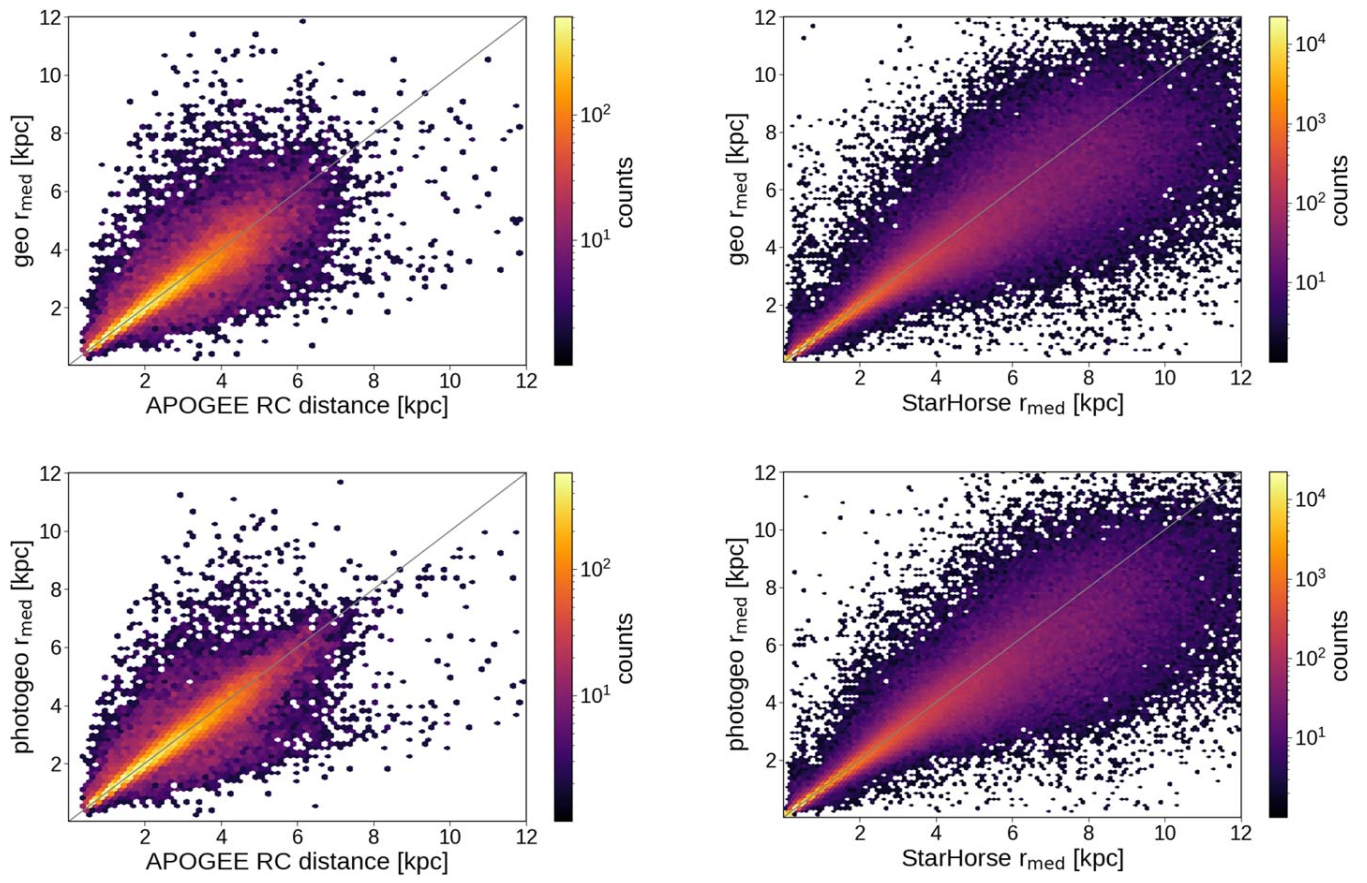
\includegraphics[width=\columnwidth]{bailerjonesverification.png}
	\caption{Comparison of Bailer Jones distances to other methods. Left: Bailer-Jones on Gaia EDR3 vs APOGEE Red Cluster (RC) measurements. Right: Bailer-Jones on Gaia EDR3 vs StarHorse Bayesean method. Top: Bailer-jones geometric method. Bottom: Bailer-Jones photogeometric method \citep{bailer-jonesEstimating2021}.}
	\label{fig:bailerjones}
\end{figure}

Ultimately Bayesian methods to improve parallax can only be as accurate as their priors and the information content of their likelihood. As a comparison to Bailer-Jones, Gaia Collaboration publishes distances derived through their General Stellar Parameterizer from Photometry (GSP-Phot)\footnote{GSP-Phot distances are available in the \texttt{distance\_gspphot} column of \texttt{gaiadr3.gaia\_source} and \texttt{gaiadr3.gaia\_source\_lite}. Additional GSP-Phot data can be found in the \texttt{gaiadr3.astrophysical\_parameters} table of the Gaia Archive}. GSP-Phot uses several priors derived from stellar models to predict stellar parameters, and then uses those stellar parameters to derive a distance. The distance itself is constrained by a geometric prior similar to the Bailer-Jones geometric prior above. This combination approach systematically underestimates distances, differing significantly from other methods past 3kpc. GSP-Phot distances do not have enough accuracy to map the Milky Way's spiral arms \citep{andraeGaia2022}.

\section{Improvement Efforts} \label{sec:improvement}

Given the state of the art of Gaia parallax distances, What should we expect in the future? Source identification is the root cause of most spurious astrometric measurements, and therefore the most likely root cause of negative and spurious parallax distances. Given that the gaia catalog has ~1.8 billion sources, this is also an extremely time consuming problem. Gaia DR4 is expected to contain more than twice the observation time as Gaia DR3, which will help reduce uncertainty driven by source selection and fitting\citep{lindegrenGaia2021a}. Comparing Gaia DR3 to the prior release, DR2, yields some striking improvements in the quality of the astrometric solutions overall.
\begin{figure}
	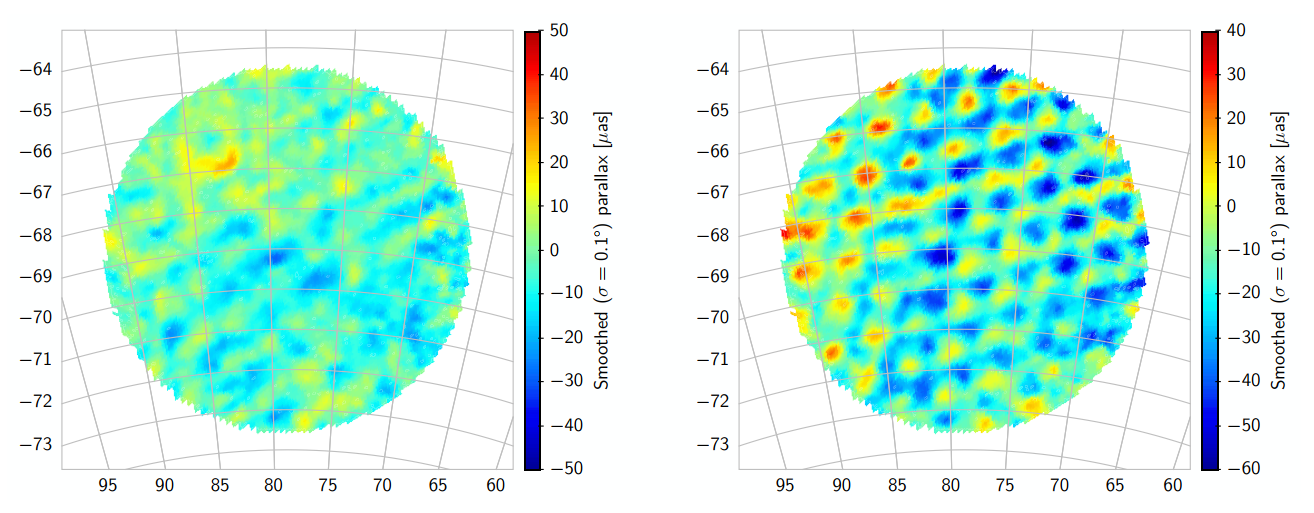
\includegraphics[width=\columnwidth]{lmcDR2vsDR3crop.png}
	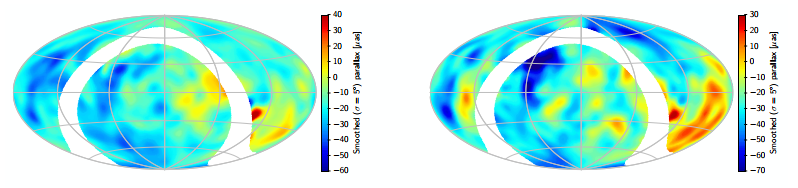
\includegraphics[width=\columnwidth]{quasarcrop.png}
	\caption{Comparison of parallaxes from Gaia DR2 (left) and Gaia EDR3 (right). Top fields show the Large Magellenic Cloud sky area. Bottom fields show distant quasars. Figures from \cite{lindegrenGaia2021a}}
	\label{fig:compare}
\end{figure}

Figure \ref{fig:compare} shows a selection of parallaxes from the Large Magellenic Cloud (LMC) and of distant quasars, with negative parallaxes appearing in red. The reduction in the waffle pattern of systemic errors in the LMC view, as well as the overall reduction in red in both diagrams shows the striking difference that additional data collection can make. Researchers estimate that the sensitivity limits of the Gaia mission as a whole are still quite far off in Gaia DR3, and that in general uncertanties will be reduced by a factor of 0.7 for positions and parallaxes, and a factor of 0.35 for proper motions\citep{lindegrenGaia2021a}. 
\begin{figure}
	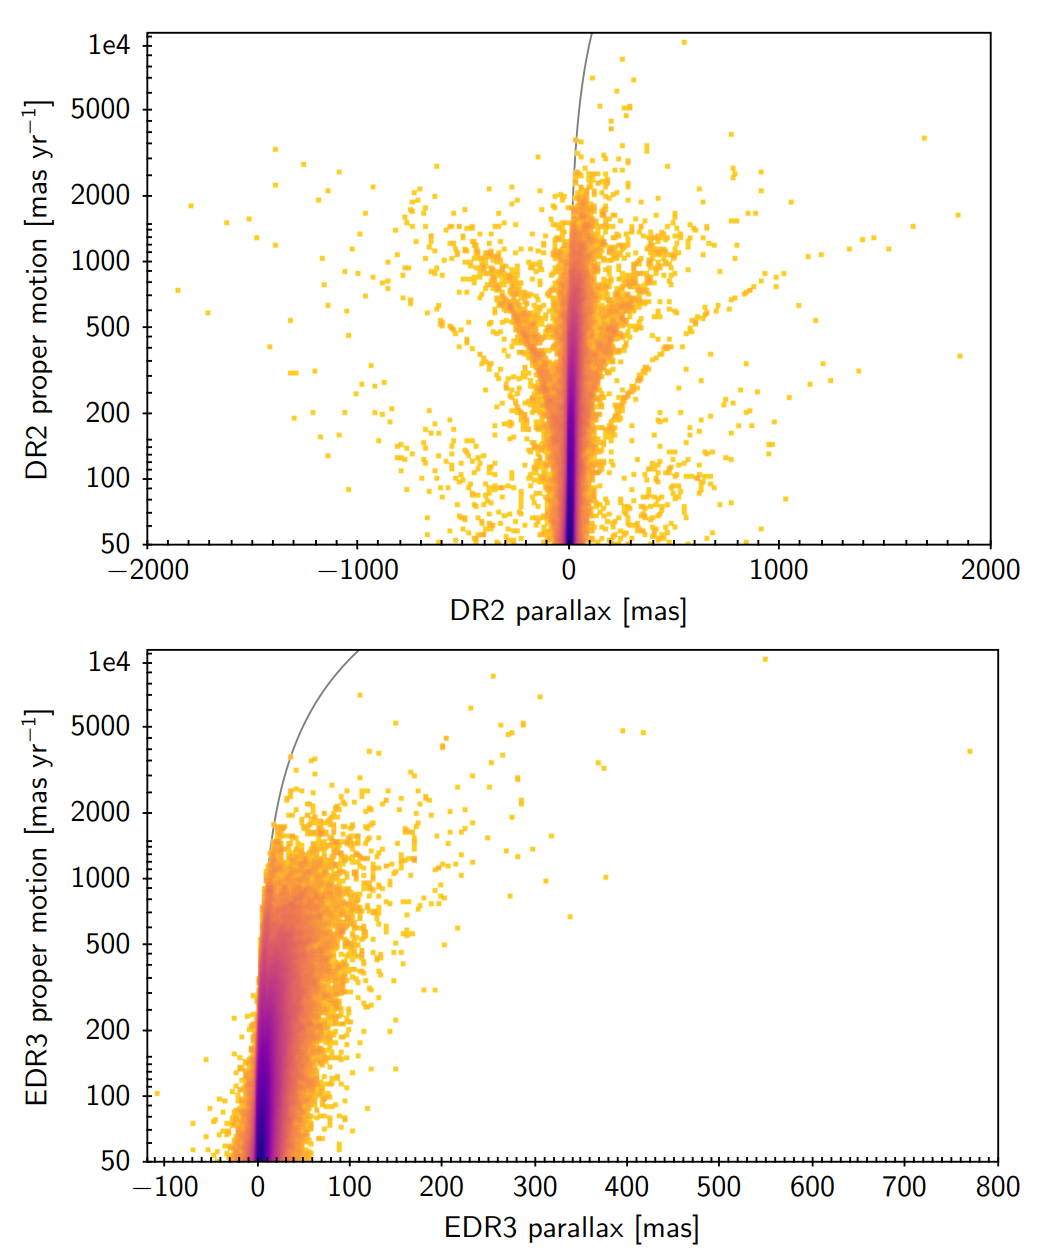
\includegraphics[width=\columnwidth]{parallaxvspropermotiondr2edr3crop.png}
	\caption{Proper motion vs parallax for DR2 (top) and EDR3 (bottom) \cite{fabriciusGaia2021}.}
	\label{fig:comparepm}
\end{figure}

The overall increase in quality of the astrometric solution between DR2 and DR3 can also be seen in the parallax and proper motions shown in figure \ref{fig:comparepm}. With parallax and proper motion coming out of the same curve fit, it is not uncommon for errors affecting one to affect the other. Figure \ref{fig:comparepm} shows the redistribution of negative parallax sources with high proper motion measured in DR2 to lower proper motion and positive parallax in EDR3. There is also a general reduction in spurious high proper motions solutions between DR2 and EDR3, corresponding to higher data quality.

\section{Unorthodox use of the astrometric solution} \label{sec:unorthodox}

The straightforward processing and curve fitting in the preparation of the astrometric values, while preserving spurious and obviously nonphysical values has a great deal of scientific value. From this data it is possible to see the effect of greater observation time on the instrument. It is also possible to prepare distance values that use even the spurious solutions to extract data about the universe. To the careful investigator, Gaia's willingness to publish their catalog while it is still in progress can enable some truly unorthodox uses of the astrometric parameters and their uncertanties.

\begin{figure}
	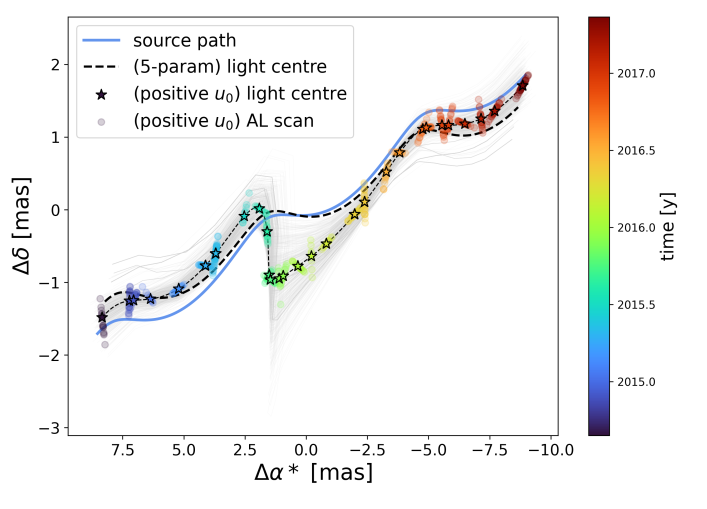
\includegraphics[width=\columnwidth]{microlensingpath.png}
	\caption{Figure from \cite{jablonskaThere2022} showing the path of the lensed object in the sky perturbed from its linear motion by a lensing event.}
	\label{fig:starpath}
\end{figure}

Researchers conjectured that the sky path of the brightest microlensing event in Gaia's database would have been altered by the lensing object as shown in figure \ref{fig:starpath} \citep{jablonskaThere2022} . In Gaia DR3 the input star locations to the astrometric pipeline are not published; however, this assumption was still validated using the astrometric parameters. \cite{jablonskaThere2022} also reports that their method allowed some limits to be placed on the mass ($M_L$), distance ($D_L$), and Einstein radius ($\theta_E$) of the lensing object. 

\cite{jablonskaThere2022} simulated gaia astrometric processing of the lensing event. These simulations varied trajectories of both objects, distance of the lensing object from earth, and the mass of the lensing object. These simulations each output the 5 astrometric parameters gaia outputs, along with uncertainties. Comparing these simulated values to the real Gaia astrometry of the lensed object, they were able to derive limits on the lensing object's properties. The simulations are scatter plotted in figure \ref{fig:simulation}, where the colors represent inclusion of a subset of the simulations based on nearness of the simulated astrometric processing errors and values to the reported Gaia values \citep{jablonskaThere2022}. They ultimately concluded that the most likely scenario was that the lensing object was a previously unknown white dwarf of approximately $~1 M_\odot$ a little less than $1 kpc$ from earth.

\begin{figure}
	\includegraphics[width=\columnwidth]{microlensingsimMD.png}
	\includegraphics[width=\columnwidth]{microlensingsimTheta.png}
	\caption{Figure from \cite{jablonskaThere2022} showing one possible set of parameters for a lensing object narrowed down from several thousand simulations}
	\label{fig:simulation}
\end{figure}

\begin{acknowledgements}
Thanks to Jim Davenport for giving a truly excellent and informative Galaxies class that reminded me of all the messy curiosity, drama, and general insanity that I appreciate about the sciences. I'd also like to thank Jake Kurlander for the first citation of my academic career, given shortly after the precursor presentation to this paper. Thanks finally and most importantly to my wife Rose Maynes for her unending support of my academic endeavours.
\end{acknowledgements}


%% For this sample we use BibTeX plus aasjournals.bst to generate the
%% the bibliography. The sample631.bib file was populated from ADS. To
%% get the citations to show in the compiled file do the following:
%%
%% pdflatex sample631.tex
%% bibtext sample631
%% pdflatex sample631.tex
%% pdflatex sample631.tex

\bibliography{finalpaper}{}
\bibliographystyle{aasjournal}

%% This command is needed to show the entire author+affiliation list when
%% the collaboration and author truncation commands are used.  It has to
%% go at the end of the manuscript.
%\allauthors

%% Include this line if you are using the \added, \replaced, \deleted
%% commands to see a summary list of all changes at the end of the article.
%\listofchanges

\end{document}

% End of file `sample631.tex'.
